\documentclass{article}
%\usepackage{apacite}
\usepackage{listings}
\usepackage{tikz}
\usepackage{pgfplots}
\usepackage{pdfpages}
\usepackage{wrapfig}
\usepackage{amsmath}
\usepackage{svg}
\usepackage{xcolor}
\usepackage{cleveref}
\usepackage{url}

\definecolor{codegreen}{rgb}{0,0.6,0}
\definecolor{codegray}{rgb}{0.5,0.5,0.5}
\definecolor{codepurple}{rgb}{0.58,0,0.82}
\definecolor{backcolour}{rgb}{0.95,0.95,0.92}

\lstdefinestyle{mystyle}{
    backgroundcolor=\color{backcolour},   
    commentstyle=\color{codegreen},
    keywordstyle=\color{magenta},
    numberstyle=\tiny\color{codegray},
    stringstyle=\color{codepurple},
    basicstyle=\ttfamily\footnotesize,
    breakatwhitespace=false,         
    breaklines=true,                 
    captionpos=b,                    
    keepspaces=true,                 
    numbers=left,                    
    numbersep=5pt,                  
    showspaces=false,                
    showstringspaces=false,
    showtabs=false,                  
    tabsize=2
}

\lstset{style=mystyle}


\usetikzlibrary{patterns}
\pgfplotsset{compat=1.18}
\svgsetup{inkscapelatex=false}
\usepackage{graphicx} % Required for inserting images

\title{Shape expressions, reification and a precious mule: building digital editions of medieval charters using the semantic web}
\author{Ángel García Menéndez}
\date{September 2026}

\begin{document}

\maketitle

\begin{abstract}
An important contribution of technology to those working with historical texts is the possibility of creating digital editions of those texts and making them available on the internet.
These editions, in contrast to traditional paper editions, can structure the information so that it can be processed by computers.
This opens up the possibility of making those editions part of the semantic web ecosystem and aligning them to the Linked Open Data principles.
To achieve this objective, we propose a methodology to integrate different semantic technologies to produce diplomatic digital editions of medieval charters.
Information in those editions will be structured using OWL ontologies, represented with RDF triples to construct a knowledge graph, validated and modeled using Shape Expressions and retrieved with SPARQL queries.
The most recent advances in semantic web technologies have also been taken into consideration. In particular, RDF 1.2 reification is used to indicate provenance and shape expressions inheritance allows to align the shapes with the classes in the ontology in a precise way.
To demonstrate the potential of this methodology, we have modeled the archive of notarial deeds from a medieval goldsmith, showing not only that it is feasible but also that it also allows for richer knowledge to be extracted from these editions and, most importantly, to combine them with other data available online.
We outline future lines of work based on the experience modeling the dataset.
Mainly, to ease some of the more time-consuming tasks via natural language processing and to create tools that would allow the non-technical user to create editions using these technologies.
\end{abstract}

\section{Introduction}

Almost since its inception, computers have served as tools to aid different types of researchers, across several disciplines.
The humanities are no exception to this, as computers first served as a support element for traditional techniques, then evolved into numerical and data analysis and, currently, putting the full potential of technology to work in what has become known as digital humanities\cite{peponaskis2024history}.

Each branch of the humanities has found different uses for technological advances\cite{dalbello2011genealogy}, and historical texts are no exception.
Palaeography, for example, has followed its own path towards digitalization,  ranging from mere representation to computational manipulation\cite{ciula_digital_2017}
That is also the case of diplomatics, another approach to the study of historical texts, which has undergone its own relationship with computers\cite{calleja2023ordenador}\cite{ambrosio:hal-02305765}.
Not to be confused with diplomacy, both disciplines derive their names from the Greek word \emph{diploma}, diplomatics is the study of the tradition, form and preparation of written acts, with the purpose of criticizing and publishing them, as defined by the Voacabulaire international de la diplomatique\cite{carcel_orti_vocabulaire_1997}.

One of the ways in which this intersection between the computer and diplomatic research has materialized is the possibility of creating digital diplomatic editions of charters.
This idea can range from the mere publication of the information online for human consultation (the case of the Digitale Charterbank Nederland\cite{burgers_digitale_2025}) to structured information fit for computer processing.
Several portals exist that offer this feature, such as Monasterium.net in Austria or the École nationale des chartes in France.
The \emph{de facto} standard for publishing these digital editions is the Text Encoding Initiative markup language\cite{tei_guidelines}.
 Although this format allows one to structure the information and even query it using XPATH, it presents two main limitations.
Firstly, it is merely a mark up representation of traditional editions, still presenting the information in a human-centered way. Secondly, they rarely link their information to the outside world.

Information is published for both transparency and, mainly, to make it available to others.
This is the main point behind Open Data.
And, to facilitate this endeavour, the World Wide Web Consortium (W3C) recommends in their star tier classification of open data that information should be linked, so that datasets can be easily integrated with each other \cite{berners-lee_linked_nodate}.
Specifically for digital humanities information, making it findable, descriptive, processable and interoperable is a key part of adding value to the data\cite{jian2026data}.
However, even though there has been a push by national libraries and archives for marking their data LOD\cite{candela2023lod}, there is still work to be done regarding medieval documents.
The Medieval Academy of America maintains a curated repository of useful sites for research, most of them containing this kind of sources\footnote{Available here: \url{https://mdr-maa.org/} (Accessed on 2026-07-15)}.
Using its filters, it is possible to see that, out of the 251 websites, 43 offer downloadable data of some kind, but only 9 have some kind of LOD feature at the moment of writing.
Plus, the 4-star tier requires the use of W3C standardized technologies, which is not common in the field of digital diplomatics, dominated by the TEI specification (not a W3C technology).
Even though there are attempts to combine both approaches\cite{vujosevic_encoding_2026}, there are still plenty of opportunities open to study the application of semantic technologies and knowledge graphs to digital diplomatics,
in terms of integration with other data and better representation and retrieval of information\cite{garcia-menendez_unlocking_nodate}\cite{burrows_linked_2022}.

The main contribution of this paper is \textbf{the proposal of an approach for the production of digital diplomatic editions of medieval charters using the range of technologies offered by the semantic web}\cite{merono2015semantic}.
The rest of the paper is structured as follows: section \ref{related-work} will provide a general overview of the state of the art regarding the publication of medieval manuscripts and the use of the semantic web.
Section \ref{methodology} explains the methodology followed and the decisions taken.
Section \ref{use-case} provides a real example of the application of the proposed methodology to an already existing data set, further discussed in section \ref{conclusion}, with limitations and possible future lines of work assessed in section \ref{future}.

\section{Related work}
\label{related-work}

Semantic web technologies and knowledge graphs have been playing a major role in modeling cultural heritage data for quite some time\cite{oneill_digital_2022}, across different domains.
There are knowledge graphs for information about Italian history\cite{carriero2019italy}, cultural heritage in Quebec\cite{marchand2020french}  or the holocaust\cite{herminio2023holocaust}, the latter using the Records in Context ontology, an alternative to CIDOC-CRM focused on archival records.
Nonetheless, CIDOC-CRM is generally the main option\cite{10.1145/3771098}, as it can be extended to accommodate information from maritime history\cite{fafalios2023sealit}, the Dutch East India Company\cite{van_wissen_2024_14065407} or conservation and restoration\cite{bannour2018crmcr}.
It is almost mandatory to talk about the SAMPO model\cite{hyvonen_digital_2023}, which provides an ecosystem to build and exploit knowledge graphs of all kinds, ranging from WWII documentation to legislation \cite{hyvonen-et-al-lawsampo-2021}, parliamentary activity\cite{hyvonen_finnish_2022}, archaeology\cite{rantala-et-al-findsampo-dhnb-2022} and library information\cite{ahola2025booksampo}.

Another group that actively promotes semantic and LOD principles in the humanities is the Pelagios Network, an association of individuals, groups and organizations focusing on producing, sharing and using historical data.
They have produced tools and methodologies to achieve these goals, as well as endorsing and sponsoring projects in diverse fields, including archaeology, geography or collections\footnote{More information: https://pelagios.org/lod/case-studies}.
Similarly, the European Union offers the Europeana Portal to serve as a library that aggregates of the common European cultural heritage.

Focusing on medieval manuscripts in particular, there are also many projects that integrate knowledge graphs to work with them.
The Mapping Manuscript Migrations Project used CIDOC-CRM and other semantic technologies to integrate information from more than 20.000 manuscripts, proving the potential of knowledge graphs and LOD in this field\cite{koho2022mmm}.
Furthermore, there is growing interest in coordinating the well established use of TEI with CIDOC-CRM and other ontologies\cite{eide_ontologies_2014}.
In this regard, the ManuscriptAI project is proposing both a formal ontology to represent the description of medieval manuscripts and the automation of the process\cite{boodts_manuscript-ai_2025}.

Charters can be considered a subset of manuscripts in general, and there are already examples of the application of knowledge graphs for their study.
The NotaryPedia project is one example of this, encoding the deeds present in the national archives of Malta\cite{ellul2019notarypedia}.
Similarly, the same dataset used in section \ref{use-case} was used to build a KG populated with the information about the legal actions and actors encoded, using a Wikibase instance as a back-end to provide collaborative capabilities\cite{alvarez-fidalgo_mckg_2026}, an approach similar to that of Digital Scriptorium\cite{falafios2023scriptorium}.
Considering how TEI dominates the landscape in digital editions, attempts have been made at bringing together the markup technology researchers are used to and RDF for linked data, by means of conversions between the two languages\cite{garcia_gonzalez_converting_2020}.
Another project aimed at exploring the potential of digital technologies is the From Digital to Distant Diplomatics project, whose aim is to increase the accessibility the information of these documents via technological means\footnote{Project's webpage: \url{https://didip.hypotheses.org/}}.

Event though all of these works cover different applications of technology for the study of medieval charters, none of them provides a full integration of the technologies from the semantic web nor a structured methodology for building digital editions.

\section{Methodology}
\label{methodology}

The proposed methodology for digital diplomatic editions will follow an approach similar to the one proposed by Chloe Shanon\footnote{Source: \url{https://ontologist.substack.com/p/do-you-need-an-upper-ontology}}, who argues for a lesser focus on ontology development and a higher emphasis in RDF reification and the use of shapes to create a data model:
\begin{itemize}
    \item Usage of an upper ontology, with extensions, to structure the domain of the problem
    \item RDF, with the reification capabilities of RDF 1.2, to represent the information
    \item Shapes to model and validate the knowledge graph
    \item SPARQL queries to extract information
\end{itemize}

One of the key decisions at the early stages was whether to create a new ontology that would fit the specific needs of the problem or whether it was possible to reuse certain vocabularies.
To approach the decision, the NeOn Methodology for ontology building\cite{suarez-figueroa_neon_2010} was used to guide the process.
Key terms of the domain were identified and different services were used to find vocabularies that contain those terms.
The most suitable alternative found and the one chosen was CIDOC's Conceptual Reference Model (CIDOC-CRM).

CIDOC-CRM is an upper ontology that serves as a general framework to build knowledge graphs related to Galleries, Libraries, Archives and Museums (GLAM)\cite{biagetti_cidoc_2016}.
Additionally, it has become an ISO standard for the interchange of cultural heritage information\cite{noauthor_iso_nodate}, making it the most suitable candidate.
This is further reinforced by the range of similar cultural heritage projects that make use of the model, as stated in section\ref{related-work}.
Another interesting advantage of CIDOC-CRM is its ecosystem of compatible models that further extend it to suit the needs of certain domains.
One of them is CRMtex, which includes several new classes and properties suitable to represent information about ancient texts\cite{doerr2020crmtex}.

There are two possible approaches to the use of CIDOC-CRM in a certain scenario: extend the ontology with new classes that specialize the model or use the E55 Type class to express the specifics of your domain.
The former approach was taken, to showcase the potential of one of the main elements of the semantic web: ontology engineering.
Ontology engineering, when done properly and based on real life well-established knowledge, is a valuable tool in the semantic ecosystem that can enrich a data model in a way that might not be possible when limited to an upper ontology.
In this particular case, the use of an upper ontology as a foundation provides a basic structure and model, which can then be easily extended and enriched by adding the domain specific classes and properties.
Thus, the resulting knowledge graphs can still be compatible and intelligible to those familiar with the upper ontology, while providing the granularity necessary for specialized research.

Firstly, a new class was added as a child of E7 Activity, the Legal Act class.
This class represents the act that the charter is recording.
Below it a whole structure of subclasses were also included, based on José Bono's book on Spanish notarial archives\cite{huerta_archivos_1985}, that represent the most common acts that might be encountered, classified in 4 categories: 

\begin{itemize}
    \item Goods, credits and services
    \item Marital affairs
    \item Testament and mortis causa liberties
    \item Personal and family
\end{itemize}

Secondly, several subclasses were added below E21 Person, to represent the different actors that might have a role in the charter: the notary, the issuer, the interventor or the scrivener.
Plus, the class Witnesses was included as a sub-class of group, representing the people that serve as witnesses in a certain legal act, as well as Notarial Document below E31 Document.
The reason for the creation of a class to represent this specific type of document was the necessity to differentiate them from other kinds of charters, such as those issued by political or ecclesiastic authorities.

Finally, several properties were added to either link the new classes with one another (e.g. recipients and granters of the act).
Most of these properties and the corresponding classes were heavily inspired by the Charters Encoding Initiative, a proposal for a new TEI module specifically designed to encode medieval charters\cite{vogeler2014cei}.
It includes tags for the main pieces of information that might be of interest when modeling the information of charters and was considered, therefore, a suitable reference.

Already in an early stage, defining the scope of the model was a challenging task.
Should it include references to locations? How should it treat relationships between people? And the role of the actors in society at the time?
It was decided to reuse existing ontologies and vocabularies as much as possible and use references to already existing resources and knowledge graphs to model specific pieces of information.
This decision, apart from easing the development of the data model, also allows the methodology to align with the Linked Open Data principles, specially the 5-star tier.
Section ~\ref{use-case} offers several examples of this, such as Wikidata for real world elements or schema.org for personal relationships.

This expanded CIDOC-CRM model offers us the basic building blocks to build a KG.
However, the specific way in which the information is represented, to serve as a system for diplomatic editions, is set via Shape Expressions (ShEx).

ShEx is a language to create grammars that indicate how a KG is constructed: which properties certain kinds of nodes may have, their cardinalities and other restrictions\cite{shex}.
These rules constitute shapes and, even though their primary purpose is validation, they can also be used to model the knowledge graph, to indicate how it should be structured.
Additionally, the latest version of ShEx includes inheritance mechanisms\cite{boneva_inheritance_2025}, similar to those of object oriented programming, providing a richer range of possibilities to model the information.

Another recent addition to the semantic ecosystem is the reification capabilities of RDF 1.2\cite{rdf1.2_2026}.
It allows the creation of triples on which the subject is another triple itself, and therefore to make statements about statements, providing additional information or context.
This is particularity useful for historical analysis, where statements may not be universal truths, but informed analysis made by experts, or they might come from specific sources.
Reification provides a mechanism to account for this provenance of the information, and has been used in this work.
For instance, instead of stating the transcription of the document as a fact, the triple linking the document to the transcription is reified to state the particular person who made the transcription and when it was carried out.

Finally, the retrieval of information, one of the key points of digital editions with structured data, is performed using SPARQL, the RDF query language.
On the one hand, the use of SPARQL over properly constructed knowledge graphs adds more and richer options than the alternative use of XPATH over TEI files.
On the other hand, by using the aforementioned external identifiers it is possible to construct federated queries and, in doing so, harness the whole potential of the semantic web and linked data.


\section{Use-case: the archive of 16\textsuperscript{th} century goldsmith Alfonso Fernández}
\label{use-case}
The methodology described in the previous section has been applied to the notarized deeds related to Alfonso Fernández, a 16\textsuperscript{th} century goldsmith from Oviedo, northern Spain. 
That archive was already analyzed and published in a PhD thesis~\cite{felpeto_cueva_archivo_2023}, for which the source documents were transcribed and compiled in 128 XML-TEI based files.
Tags were used to delimit the different elements of the diplomatic analysis in the transcription of the text, and the different actors were identified, along with a brief description of the legal action encoded in each particular document and different pieces of metadata, such as physical information about the original document or relevant locations.
Nonetheless, much of that information was either expressed as blocks of text in natural language or not linked to any external sources to facilitate its reuse.

That dataset, with permission from its original authors, was manually converted into an RDF-based representation following the methodology proposed in section \ref{methodology}\footnote{To preserve anonymity during peer review, the dataset has been uploaded as a resource in the submission. Upon acceptance, the data will be transitioned to a permanent, citable archive}.
The resulting knowledge graph was composed of 24.989 triples and used classes and properties from our custom extension of CIDOC-CRM and CRMtex, alongside some properties and classes borrowed from schema.org (personal information of actors)\cite{guha2016schema}, agrelon (family relations)\cite{litz2012agrelon} and VID (diplomatic elements). References to Wikidata were used to link certain entities or types in general and, in the specific case of locations, references to the Geographic Thesaurus from the Spanish Ministry of Culture (published in SKOS and available through an SPARQL endpoint) were employed.

Three main pieces of information should be encoded per document: the transcription, the diplomatic analysis of the text and the real life information that the document encoded.
This first element is achieved using a node of type E34 Inscription with a note using the P3 has note property pointing to the whole transcription.
The analysis of the text, both of its physical characteristics as a manuscript and its diplomatic elements, is modeled using a node of type TX1 Written Text.
The class Diplomatic Element was added to the ontology, as a child of TX7 Written Text Segment.
Each of the portions of text that are deemed significant for the analysis are described using a node of this type, plus a reference to the online version of the Vocabulaire international de la diplomatique (VID), published as a thesaurus of terms in SKOS\footnote{Available here: \url{https://www.cei.lmu.de/VID/skos/}}.
Finally, each document references the Legal Act that it records, for which the various actors are linked, along with the object of the contract and other pieces of information, depending on the specific type of act.

To illustrate this, on appendix \ref{comparison} we can see an extract from file AMSPO\_FSV\_1612.xml.
It offers a natural language description of the legal act that the charter encodes and then several pieces of structured information, such as the date, participants, type of act or object in the transaction.
Even though some of that information can be queried, interesting details such as the relationships between the participants is only present in natural language.
Plus, data such as professions or the object being sold is represented as string literals.
In the same appendix we may find the diagram describing the sub-graph corresponding to that very same data.
The starting point is the node representing the particular document, which is said to document an act, which then links to the different its different elements.
The object, even though it still stores its human readable description, uses the Wikidata entity 
Similarly, the location points to the corresponding entry in the geographic thesaurus.
And, for each of the actors, their personal information, relationships and occupations are present, the latter using URIs from Wikidata, allowing to retrieve information from that source.

\begin{figure}
    \centering
    \includesvg[width=\textwidth]{diagram}
    \caption{Simplified class diagram of the shape expression schema. Titles in the boxes indicate the name of the shape, and the text in italics indicates the type (rdfs:type) of the node that the shape applies to.}
    \label{somier}
\end{figure}

The ShEx schema developed to both validate and model the knowledge graph is composed of 25 shapes (see figure \ref{somier} for a summarized class diagram).
The \texttt{Act} shape, which represents the legal act recorded in the document, stores the basic information of any act (granter and recipient, who notarizes the document, where and when it took place).
This shape is then extended using ShEx inheritance to add information about the specific acts present in the dataset, such as total price for sales or the periodicity of payments in rentals.
Therefore, it is possible to both filter the acts by their types as specified by the ontology, to ensure that all of them encode the basic information expected in all acts and to include the details specific to each particular type, without affecting the rest and maintaining the consistency of the model.
A similar strategy is followed with the \texttt{Person} shape, which is extended by \texttt{Notary} and \texttt{Amanuensis} to add the specific pieces of information regarding those types of nodes.

Two main types of information were considered suitable candidates for the use of RDF 1.2 reification.
Firstly, the three pieces of information for each document include a reified statement, indicating the researcher who performed the analysis of that information and the date on which it was done, by means of the Provenance, Authoring and Versioning ontology\cite{ciccarese_pav_2013}.
Secondly, a total of 291 individuals were identified in the dataset.
Apart from their full name and gender, several other pieces of information about each person could be extracted from the document, such as occupation, residence of family relations.
Those statements were reified, indicating the source document of that data by means of the source property from the Dublin Core Metadata Terms vocabulary.
Therefore, any future researcher could, not only check the information of the individual, but also trace back the original text where that information is stated.

To validate the model, as stated in section \ref{methodology}, several competency questions were created along with a team of researchers specialized in historical documents and digital humanities.
A total of 42 questions were first introduced in natural language and, once the dataset was complete, translated into SPARQL queries.
The CQ can be divided into 4 categories:
\begin{itemize}
    \item Metadata: questions regarding information about the document, such as its physical location, dimension or identifier.
    \item Entities: questions regarding the entities of the document, such as the legal act being recorded, its participants or the object that is referenced in the act.
    \item Structure: questions about the structure of the text in the diplomatic sense, such as its legal formulas or the clauses present in the contract
    \item Grouping: questions of a more complex nature, that require the aggregation and grouping of data in order to extract results
\end{itemize}

All competency questions could be answered using the model.
Grouping questions are especially interesting, as they could not be easily expressed using XPATH, which was the method previously used with the TEI-based representation.
For example, to the competency question \texttt{RFG-01} \emph{List all notaries in the corpus, along with their first appearance date and the total number of documents they notarized} the SPARQL query in listing  \ref{rfg-01} was proposed

\begin{lstlisting}[language=SPARQL, label={rfg-01}, caption=SPARQL query corresponding to competency question \texttt{RFG-01}]
SELECT DISTINCT ?notary ?firstName ?lastName
       (MIN(?documentDate) AS ?firstAppearance)
       (COUNT(DISTINCT ?document) AS ?totalDocuments)
WHERE {
  ?document a dip:Notarial_Document ;
            crm:P70_documents ?legalAct ;

  ?legalAct dip:is_notarized_by ?notary .

  ?notary schema:givenName ?firstName ;
          schema:familyName ?lastName .

  ?document crm:P128i_is_caried_by ?text .
  ?text crm:P4_has_time_span ?timeSpan .
  ?timeSpan crm:P170i_time_is_defined_by ?documentDate .
}
GROUP BY ?notary ?firstName ?lastName
ORDER BY ASC(?firstAppearance)
\end{lstlisting}

Plus, other questions could be answered only by means of federation with external SPARQL endpoints.
Question \texttt{RFEN-06} requires determining whether a person is part of the clergy or not.
Instead of modeling that information into the KG, each person's occupation was linked to its corresponding Wikidata entity.
Using federation allowed to check whether that equivalent Wikidata entity was a subclass of P279 (religious figure). 
The resulting distribution can be observed in figure \ref{fig:granters}.

The chosen tool to perform all the manipulation of the KG, both in terms of validation and querying, was the Rudof library for the manipulation of RDF and shapes, implemented in Rust\cite{labra-gayo_rudof_nodate}.
The reasons for this choice were mainly two.
Firstly, it provides an implementation for the most recent characteristics of the RDF ecosystem, namely RDF 1.2 and ShEx inheritance, while maintaining a competitive performance.
Secondly, thanks to its Python Bindings, the data and the scripts can be published online in a self-contained manner, as only the specific version of the library is required to replicate the results.

\begin{wrapfigure}{r}{0.55\textwidth}
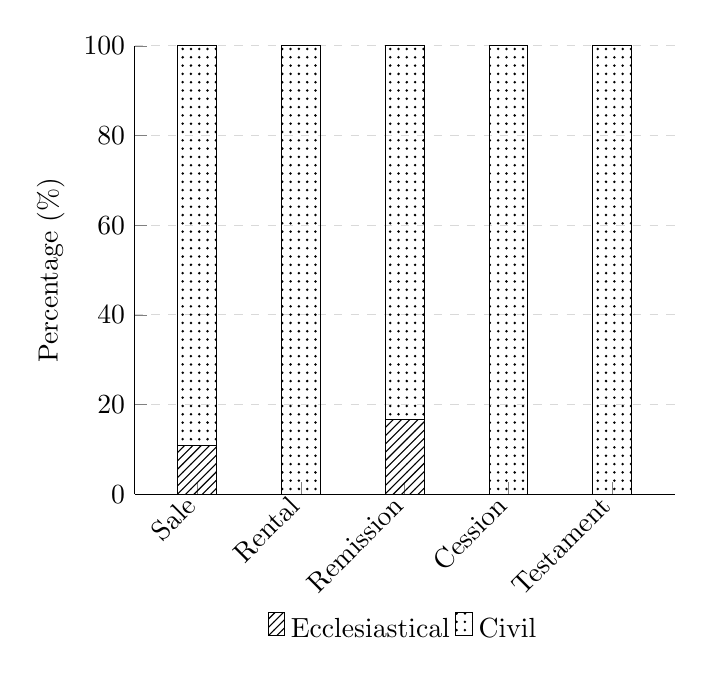
\begin{tikzpicture}
\begin{axis}[
    ybar stacked,
    bar width=14pt,
    ymin=0,
    ymax=100,
    ylabel={Percentage (\%)},
    symbolic x coords={Sale,Rental,Remission,Cession,Testament},
    xtick=data,
    xticklabel style={
        rotate=45,
        anchor=east
    },
    axis x line*=bottom,
    axis y line*=left,
    enlarge x limits=0.15,
    legend style={
        at={(0.5,-0.25)},
        anchor=north,
        legend columns=2,
        draw=none
    },
    ymajorgrids=true,
    grid style={dashed,gray!30}
]

% Ecclesiastical
\addplot[pattern=north east lines] coordinates {
(Sale,10.81)
(Rental,0)
(Remission,16.67)
(Cession,0)
(Testament,0)
};

% Civil
\addplot[pattern=dots] coordinates {
(Sale,89.19)
(Rental,100)
(Remission,83.33)
(Cession,100)
(Testament,100)
};

\legend{Ecclesiastical,Civil}

\end{axis}
\end{tikzpicture}
\caption{Percentage of ecclesiastical and civil granters, distributed by the type of legal act}
\label{fig:granters}
\end{wrapfigure}


\section{Conclusions}
\label{conclusions}

The framework presented in this paper brings together the power of the full ecosystem of the semantic web into a field of research to which it had only been partially applied.
With this example we are able to show how it can be used by diplomatists to build digital editions of charters.
There are ontological frameworks to represent the information contained in medieval charters and they can be extended to meet the domain demands.
RDF makes it possible to structure information closer to real knowledge and, thanks to reification, maintain accountability for the origin of said information, which in turn can be explored and merged with other data via SPARQL.
The integrity of the data can be guaranteed by means of ShEX, whose shapes can be aligned to the structure of the ontology thanks to inheritance.

Furthermore, this semantic approach aligns the traditional goals of diplomatic editions with those of the semantic web.
Unlike traditional editions, confined to physical books, and digital editions which merely rely on pouring those same contents online, RDF and knowledge graphs make the information in these charters reusable via machines and connects it with other data, making them part of the global web of linked open data.
Reaching the 5 stars in the LOD is not a goal in and of itself, but the necessary step towards making this data interoperable and discoverable, therefore contributing to future research and uses of the data in ways we may not currently see.

However, even when the data is used on its own, this representation offers new possibilities.
Exploring personal relations among the actors, how the structure of the texts changes and evolves across notarial offices, and the implications of the locations which are referenced in the texts are all plausible scenarios for the potential to retrieve and process information from charters.

Finally, the methodology presented in this work aims to be adaptable to different realities.
Even though its focus is in the European tradition of charters, information from other countries may be expressed using the methods and techniques described.
The level of detail with which the legal acts are represented is specifically chosen to accommodate different kinds of events, taking into account only the generic legal roles of the actors.
Therefore, should a diplomatist from another country wish to use their own hierarchy to encode specific types of acts, doing so would be trivial.
Similarly, all the types of diplomatic elements reference the VID, which is itself a standard for the field.
And one of the reasons for choosing CIDOC-CRM as our base framework was precisely to both make ours interoperable with other pieces of data and to model it with a common language, which anyone familiar to this standard would understand.

\section{Limitations and future work}
\label{future}
The work presented is intended to serve as a proof of concept to prove the potential of the semantic web in this particular field.
Therefore, the model was accommodated to the information present in the dataset used.
For example, even though all types of legal acts were added to the ontology, only those present in the dataset were added specific properties to fit their needs.
Moreover, we have focused on notarial charters and, therefore, left behind some characteristics that other types of charters (such as those issued by civic or religious authorities) may require.
On the other hand, the level of detail to which elements of the text are identified has been limited to those types present in the VID, while the original XML corpus included custom tags to mark up other textual elements of interest.

Although these limitations will be overcome in the future as the model becomes more complex to accommodate a wider range of document types, there are others whose solutions are not as straightforward.

There is an obvious weakness when comparing this representation with one based on TEI.
Namely, the difficulty of writing an RDF knowledge graph manually.
TEI is used here as an annotating technology, adding markup to a diplomatic edition that it is not that much different from a traditional one.
A researcher without a technical background, given some training, can be expected to add markup to the transcription of a charter, there is not a big leap in terms of abstraction.
However, our proposal requires a total change of mindset, to go from a representation centered around a text to one in which a collection of data points represents the connection between pieces of knowledge.
Even though the latter is arguably closer to the representation of that same information in the human mind, the former is more intuitive to the veteran diplomatist.
Additionally, a file structure composed of RDF triples is prone to mistakes when written directly by humans and, even with ShEx validation, detecting the source of said mistakes can prove a challenge.
The same can be said about the use of SPARQL for information retrieval.
It requires some training and experience to use SPARQL to its full potential, both in terms of understanding the syntax and how the queries themselves work.

The other limitation that should be addressed is the inefficiency of this manual process.
Not only the transcription of the text according to diplomatic rules, but also the analysis of the textual elements,  the identification of the entities and schematization of the legal act recorded in the charter.
All of these steps are time-consuming and, as stated before, prone to errors and mistakes.

These two main limitations outline the two main future lines of work.
Firstly, it would be necessary to make this methodology user friendly through a graphical editor.
Although the decision to develop one from scratch or to adapt some already existing software is to be taken in the future, it is a necessary step towards making this technological framework accessible to researchers in the humanities.
Secondly, several tasks involved in the creation of these digital editions can be automated, or at least semi-automated, to some degree.
Natural Language Processing techniques, including those considered more traditional and the LLM-based, need to be evaluated to find those that may ease the work of historical researchers with these texts.

%\begin{acks}
%This work has been partially funded by:
%\begin{itemize}
%    \item  
%    \item 
%    \item 
%\end{itemize}
%\end{acks}
  
\appendix
\section{Comparison between the TEI-based and the RDF-based representation}
\label{comparison}
\begin{lstlisting}[language=xml, label={tei}, caption={Extract from file AMSPO\_FSV\_1612, with its contents translated into English. It shows the date on which the act recorded by the charter took place, a natural language description of the act and a list of the actors involced, alongside some metadata abut the nature of the act.}]
<abstract>
    <date when="13300818" where="">
        <year>1330</year>
        <month>08</month>
        <date>18</date>
    </date>
    <p>Marcos Pelaez, chaplain of San Miguel de Bascones (Grado), sells to the goldsmith Alfonso Fernandez from Oviedo and to his wife Maria Alvarez a granary with a straw ceiling located in the cementery of said church, for a mule priced at fifty maravedi</p>
</abstract>
<encodingDesc>
    <action type="sale"/>
    <object type="granary"/>
    <person type="chaplain" role="G" sex="m">Marcos Pelaez, chaplain of San Miguel de Bascones (Grado)</person>
    <person type="particular" role="R" sex="m">Alfonso Fernandez, goldsmith</person>
    <person type="particular" role="R" sex="f">Maria Alvarez, wife of goldsmith Alfonso Fernandez</person>
</encodingDesc>
\end{lstlisting}

\begin{figure}
    \label{kg}
    \centering
    \includesvg[width=0.80\textwidth]{diagram_amspo_fsv_1612}
    \caption{Diagram representing the different nodes in the RDF-based representation of file AMSPO\_FSV\_1612. Blue nodes correspond to the local nodes of the KG. Purple nodes correspond to classes linked to the nodes by means of the rdfs:type property. Clouds represent links to resources from external KG and yellow cards contain the value of literals. The arrows represent the links between nodes by means of triples, with the name of the corresponding property stated.}
\end{figure}


\bibliographystyle{plain}
\bibliography{refs}

\end{document}
